\documentclass{beamer}
\setbeamertemplate{footline}[frame number]
\usepackage[utf8]{inputenc}

\title{Using Graph Neural Networks in Local Search for Relaxations of the Maximum Clique Problem}
\subtitle{180.773 Seminar for Master Students in Logic and Computation}
\author{Rupert Ettrich}
\date{23rd June 2022}

\begin{document}

\maketitle

\begin{frame}{Outline}
\begin{itemize}
    \item Problem Statement and Motivation
    \item Aim of the Thesis and Expected Results
    \item State of the Art
    \item Methodology
    \item Context within the Logic and Computation Master's Program
\end{itemize}
    
\end{frame}

\section{Problem Statement and Motivation}

\begin{frame}{Motivation}
    \begin{itemize}
        \item<1-> Instances of many Combinatorial Optimization Problems (COPs) exhibit clearly defined internal structures that can be expressed as graphs
        \item<2-> Growing interest in utilizing Machine Learning (ML) techniques in algorithms for COPs
        \item<3-> Graph Neural Networks (GNNs): NNs specifically tailored to learn from graph input 
    \end{itemize}
\begin{figure}
    \centering
    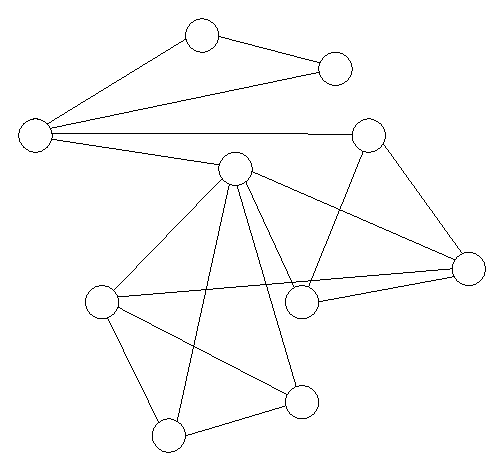
\includegraphics[width=0.3\textwidth]{graphics/graph1.eps}
\end{figure}
\end{frame}

\begin{frame}{Motivation}
    \begin{itemize}
        \item<1-> End-to-end ML approaches not competitive to leading heuristic methods
        \item<2-> Successful applications: e.g. GNN guided destroy operator in LNS \cite{Oberweger2022}
        \item<3-> Motivation: Study application of GNNs in context of (meta-)heuristics for COPs on graphs
    \end{itemize}
\end{frame}

\begin{frame}{Maximum Clique Problem}
    \begin{definition}
        Given a graph $G= (V,E)$, the Maximum Clique Problem is the problem of finding a fully connected subgraph (\textit{clique}) of maximum size in $G$.
    \end{definition}
    \begin{itemize}
        \item Decision variant is one of Karp's 21 NP-Complete problems \cite{Karp1972}
        \item Applications in bioinformatics \cite{Dognin2010}, social network analysis \cite{Pattillo_network_analysis_2013}, etc...
        \item MCP too strict a model for many real-world applications
    \end{itemize}
    \begin{figure}
        \centering
        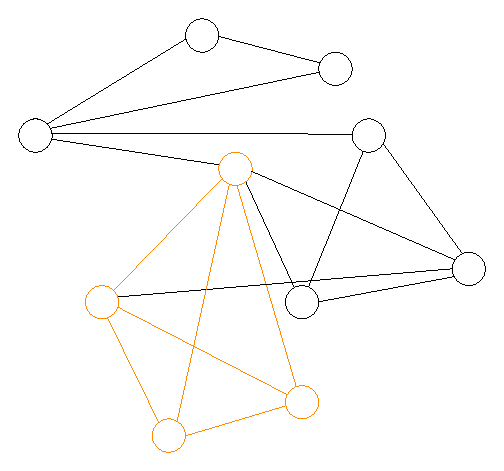
\includegraphics[width=0.3\textwidth]{graphics/graph1-clique.eps}
    \end{figure}
\end{frame}

\begin{frame}{Maximum Quasi-Clique Problem}
    \begin{definition}
	\label{def:mqcp}
	Given a graph $G = (V,E)$ and $\gamma \in (0,1]$, the Maximum $\gamma$-Quasi-Clique Problem (MQCP) is the problem of finding a subset of vertices $S \subseteq V$ of maximum size 
	such that the induced subgraph $G[S]$ has an edge density of at least $\gamma$, or, in other words, $G[S]$ contains at least $\gamma \binom{|S|}{2}$ edges. 
    \end{definition}
    \begin{itemize}
        \item Introduced in \cite{Abello2002}
        \item NP-hard for $\gamma \in (0,1]$ \cite{pattillo_maximum_2013}
    \end{itemize}
\end{frame}

\begin{frame}{Aim of the Thesis and Expected Results}
    \begin{itemize}
        \item<1-> Main goal: contribute to study of applications of GNNs in COPs
        \item<2-> Develop heuristic algorithm for relaxations of the MCP that is enhanced by a GNN
        \item<3-> Based on local search: Use GNN to guide exploration of neighborhoods
    \end{itemize}
\end{frame}

\begin{frame}{Aim of the Thesis and Expected Results}
    \begin{itemize}
        \item<1-> Consider similar applications of GNNs in COPs and explore suitable GNN architectures
        \item<2-> Develop and investigate methods for training data generation and training the GNN
        \item<3-> New heuristic solution approach that is substantially different from existing methods
        \item<4-> Hopefully lead to new research in context of GNNs in COPs
    \end{itemize}
\end{frame}

\begin{frame}{State of the Art - GNNs in COPs}
    \begin{itemize}
        \item<1-> Graph Attention Network \cite{Velickovic2018} is a prominent GNN model that translates attention mechanism \cite{Bahdanau2015} to graph-based tasks
        \item<2-> Several applications build upon this GNN model: e.g. \cite{Kool2019}, \cite{Joshi2021} (TSP)
        \item<3-> Graph Neural Network Guided Local Search for TSP: \cite{Hudson2021}: Lower optimality gaps, better generalization on larger instances
        \item<4-> ML-based methods for MCP: Pointer Network \cite{Gu2020}, Graph Convolutional Network \cite{Li2018}
        \item<5-> No approaches using GNNs for MQCP or other clique relaxations
    \end{itemize}
\end{frame}

\begin{frame}{State of the Art - Algorithms for MQCP}
    \begin{itemize}
        \item<1-> Exact methods:
        \begin{itemize}
            \item Most approaches either branch-and-bound or MILP-formulations
            \item Leading methods fail to solve very dense graphs with 100 nodes in $<$ 1 hour
        \end{itemize}
        \item<2-> Leading heuristic methods:
        \begin{itemize}
            \item Biased Random-Key Genetic Algorithm \cite{pinto_biased_2018}
            \item Adaptive Multi-Start Tabu Search \cite{djeddi_extension_2019}
            \item Opposition-Based Memetic Algorithm (uses Tabu Search) \cite{zhou_opposition-based_2020}
            \item NuQClq: Local Search with Configuration Checking and improved exploration of neighborhoods \cite{chen_nuqclq_2021}
        \end{itemize}
    \end{itemize}
\end{frame}

\begin{frame}{Methodology - Algorithm Structure}
    \begin{itemize}
        \item<1-> Approximate maximum $\gamma$-quasi clique by finding $\gamma$-quasi cliques of increasing size
        \item<2-> Move operator: Swap vertices in $S$ with vertices in $V \setminus S$
        \item<3-> Neighborhood Structure: Contains $k$-element subsets of $V$ that can be obtained by swapping $u \in S$ with $v \in V \setminus S$
    \end{itemize}
    
\begin{figure}
    \centering
    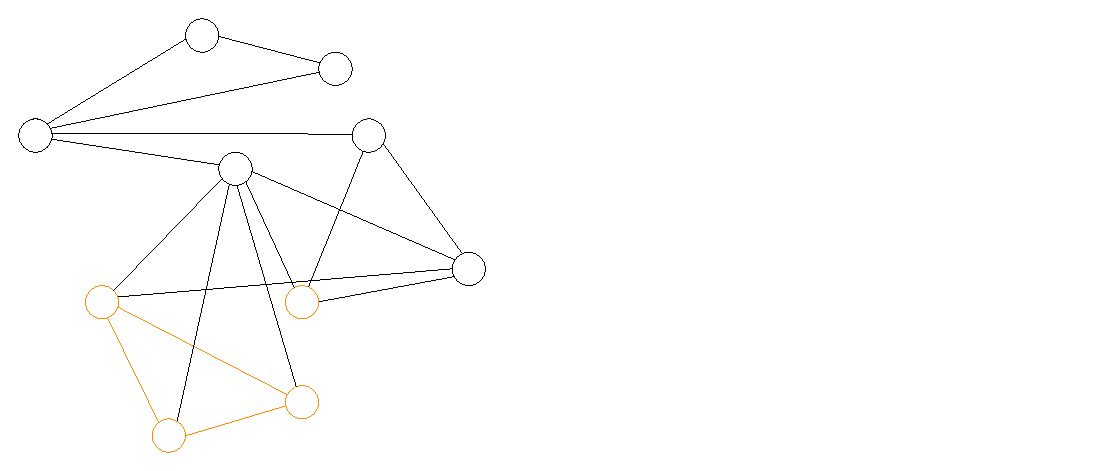
\includegraphics[width=0.7\textwidth]{graphics/graph-before-swap.eps}<4->
\end{figure}
\end{frame}

\begin{frame}{Methodology - Algorithm Structure}
    \begin{itemize}
        \item Approximate maximum $\gamma$-quasi clique by finding $\gamma$-quasi cliques of increasing size
        \item Move operator: Swap vertices in $S$ with vertices in $V \setminus S$
        \item Neighborhood Structure: Contains $k$-element subsets of $V$ that can be obtained by swapping $u \in S$ with $v \in V \setminus S$
    \end{itemize}
    
\begin{figure}
    \centering
    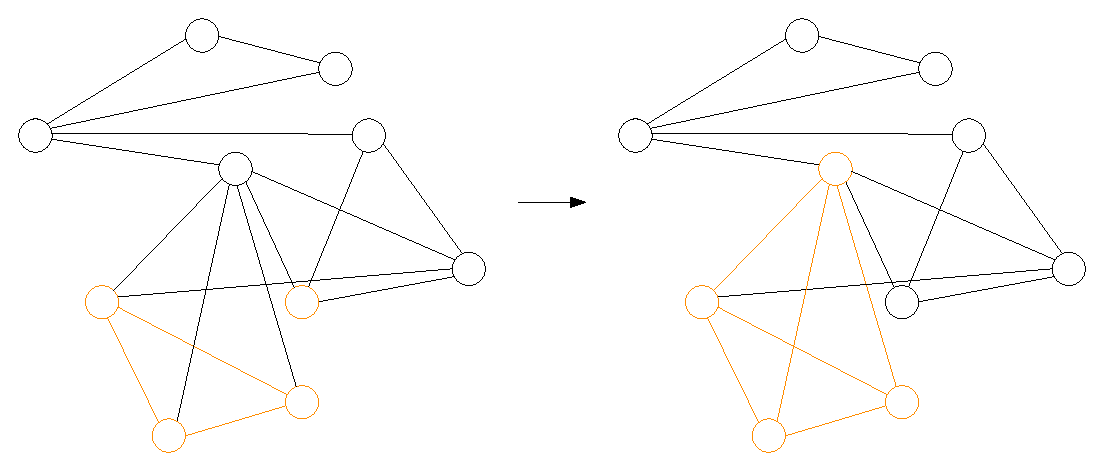
\includegraphics[width=0.7\textwidth]{graphics/graph-after-swap.eps}
\end{figure}
\end{frame}

\begin{frame}{Methodology - Algorithm Structure}
    \begin{itemize}
        \item<1-> Construction heuristic generates candidate solution $S \subset V$ with $|S| = k$
        \item<2-> Move operator: Swap vertices in $S$ with vertices in $V \setminus S$
        \item<3-> If candidate solution becomes feasible, increase $k$ and restart search
        \item<4-> Otherwise, if local optimum reached:
        \begin{itemize}
            \item If stop criterion not met: Apply diversification and restart search
            \item Otherwise: Return best found feasible solution
        \end{itemize}
    \end{itemize}
\end{frame}

\begin{frame}{Methodology - Exploring neighborhoods with GNN}
    \begin{itemize}
        \item<1-> Use pre-trained GNN to guide exploration of neighborhoods
        \item<2-> Graph Attention Networks \cite{Velickovic2018} seem promising, applications in similar scenarios
        
    \end{itemize}
\end{frame}
        

\begin{frame}{Methodology - Exploring neighborhoods with GNN}
Encoder - Decoder paradigm: 
    \begin{itemize}
            \item Capture graph structure in node embeddings and graph embedding
    \end{itemize}
    \begin{figure}
        \centering
        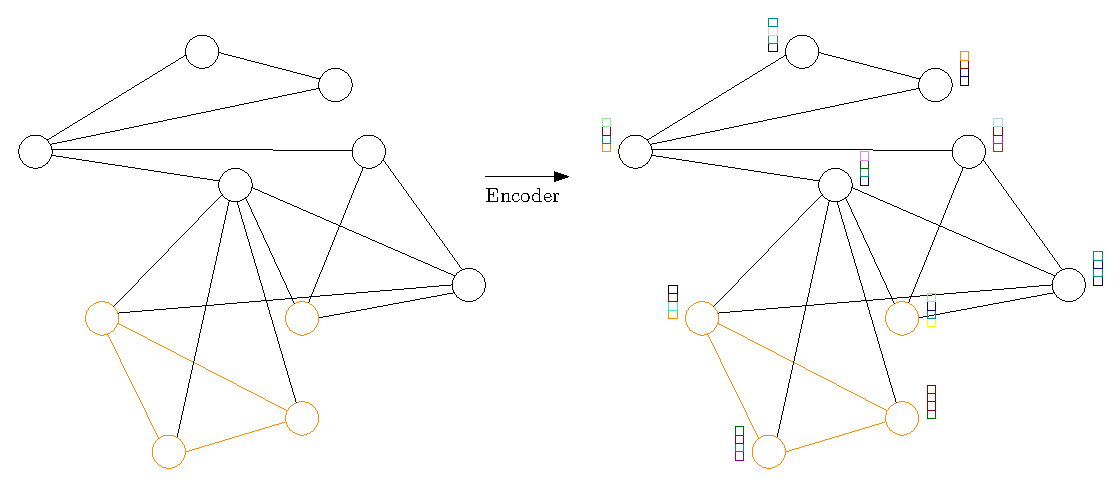
\includegraphics[width=1.0\textwidth]{graphics/graph-encoder.eps}
    \end{figure}
\end{frame}

\begin{frame}{Methodology - Exploring neighborhoods with GNN}
Encoder - Decoder paradigm: 
    \begin{itemize}
            \item Capture state (candidate solution) in context embedding
    \end{itemize}
    \begin{figure}
        \centering
        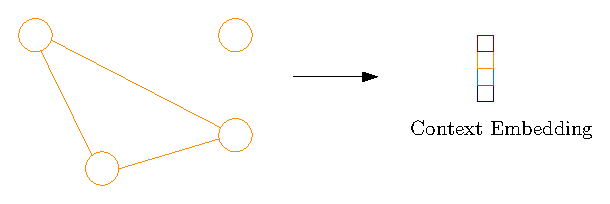
\includegraphics[width=0.7\textwidth]{graphics/graph-state.eps}
    \end{figure}
\end{frame}

\begin{frame}{Methodology - Exploring neighborhoods with GNN}
Encoder - Decoder paradigm: 
    \begin{itemize}
            \item Use Decoder to obtain scores for nodes in $G$: Consider swaps of nodes in $V \setminus S$ with high scores with nodes in $S$ with low scores 
    \end{itemize}
    \begin{figure}
        \centering
        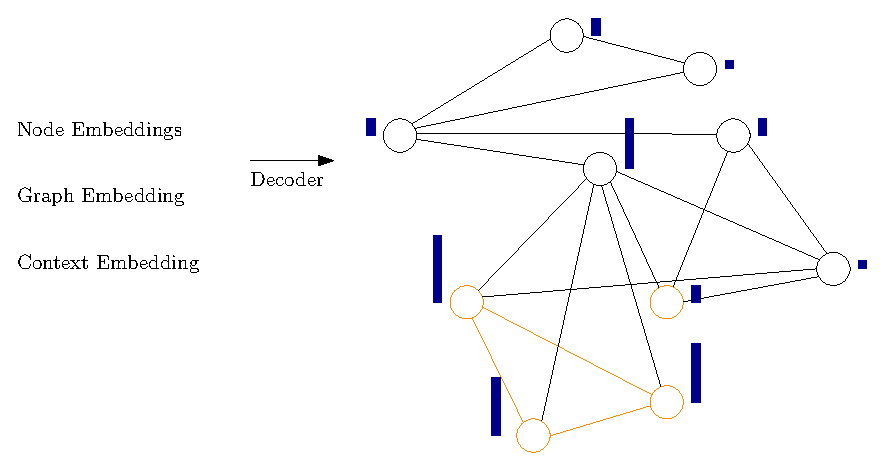
\includegraphics[width=\textwidth]{graphics/graph-decoder.eps}
    \end{figure}
\end{frame}

\begin{frame}{Methodology - Training the GNN}
    \begin{itemize}
        \item<1-> Generate representative problem instances (graphs)
        \item<2-> At random points in local search, generate training samples from
        \begin{itemize}
            \item Graph
            \item Candidate solution
        \end{itemize}
        \item<3-> Look-ahead search that finds (approximate) best solution in neighborhood after $d$ swaps is used as target
        \item<4-> Train GNN to predict higher scores for nodes that are in solution obtained by look-ahead search
        \item<5-> Find suitable hyperparameters (layers in GNN, depth $d$ of look-ahead)
    \end{itemize}
\end{frame}

\begin{frame}{Methodology - Evaluation}
    Evaluate on commonly used benchmark sets:
    \begin{itemize}
        \item DIMACS
        \item BHOSLIB
        \item Florida Sparse Matrix Collection
        \item Stanford Large Network Dataset Collection
    \end{itemize}
\end{frame}

\begin{frame}{Context within LAC Master's Program}
Relevant courses include
\begin{itemize}
	\item 186.814 Algorithmics
	\item 186.181 Algorithms in Graph Theory
	\item 186.112 Heuristic Optimization Techniques
	\item 184.702 Machine Learning
	\item 186.835 Mathematical Programming
	\item 186.820 Project in Computer Science 1
\end{itemize}
\end{frame}

\bibliographystyle{apalike} 
\bibliography{abstract-proposal}

\begin{frame}{Maximum k-defective Clique Problem}
    \begin{definition}
	\label{def:mdcp}
	Given a graph $G = (V,E)$ and integer $k$, the Maximum $k$-defective Clique Problem (MDCP) is the problem of finding a subset of vertices $S \subseteq V$ of maximum size 
	such that the induced subgraph $G[S]$ contains at least $\binom{|S|}{2} - k$ edges. 
\end{definition}
\end{frame}

\begin{frame}{Maximum k-plex Problem}
    \begin{definition}
	\label{def:mpp}
	Given a graph $G = (V,E)$ and integer $k$, the Maximum $k$-plex Problem (MPP) is the problem of finding a subset of vertices $S \subseteq V$ of maximum size 
	such that each $v \in S$ is adjacent to at least $|S| - k$ vertices in $S$. 
\end{definition}
\end{frame}

\end{document}
